% answers.tex —— 2011 年·江苏卷 · 参考答案与详细解析片段
% 由 tools/generate_projects.py 依来源总账自 2011/2011_数学真题_江苏_试题.md + 2011/2011_数学真题_江苏_解析正文.md + 2011/2011_数学真题_江苏_答案要点.md 生成，勿手改（改源 MD 后重跑）

\begin{answer}
\gksolhead{1}{}

\textbf{题目}：

已知集合 $A=\{-1,1,2,4\}$，$B=\{-1,0,2\}$，则 $A\cap B=$ $\underline{\qquad}$。

\Needspace{4\baselineskip}
\textbf{解析}
$A=\{-1,1,2,4\}$，$B=\{-1,0,2\}$，公共元素为 $-1$ 与 $2$，故 $A\cap B=\{-1,2\}$。

\gkanswer{答案：$\{-1,2\}$。}

\end{answer}
\begin{answer}
\gksolhead{2}{}

\textbf{题目}：

函数 $f(x)=\log_5(2x+1)$ 的单调增区间是 $\underline{\qquad}$。

\Needspace{4\baselineskip}
\textbf{解析}
$f(x)=\log_5(2x+1)$ 的定义域为 $2x+1>0$，即 $x>-\dfrac12$。底数 $5>1$，对数函数在定义域上单调递增；内层 $2x+1$ 也递增，故单调增区间为 $\left(-\dfrac12,+\infty\right)$。

\gkanswer{答案：$\left(-\dfrac12,+\infty\right)$。}

\end{answer}
\begin{answer}
\gksolhead{3}{}

\textbf{题目}：

设复数 $z$ 满足 $\mathrm i(z+1)=-3+2\mathrm i$（$\mathrm i$ 是虚数单位），则 $z$ 的实部是 $\underline{\qquad}$。

\Needspace{4\baselineskip}
\textbf{解析}
\Needspace{5\baselineskip}
$\mathrm i(z+1)=-3+2\mathrm i$，两边除以 $\mathrm i$：
\nopagebreak[4]
\[z+1=\frac{-3+2\mathrm i}{\mathrm i}=(-3+2\mathrm i)(-\mathrm i)=2+3\mathrm i,\]
故 $z=1+3\mathrm i$，实部为 $1$。

\gkanswer{答案：$1$。}

\end{answer}
\begin{answer}
\gksolhead{4}{}

\textbf{题目}：

根据如图所示的伪代码，当输入 $a$，$b$ 分别为 $2$，$3$ 时，最后输出的 $m$ 的值是 $\underline{\qquad}$。
\nopagebreak[4]
\begin{center}% 2011 年江苏卷第 4 题：伪代码。
% 来源 PDF：普通高考/2011/2011江苏.pdf，SHA-256 71763ef5d0c2b5800c12515e6b3addb77e585b2460fd11c1013fcec6f050ece9。
% 原页：第 1 页第 1 栏，书页码 675。照原页逐行重排。
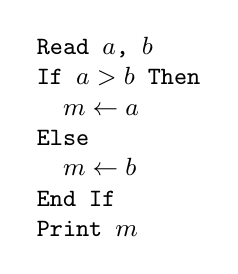
\begin{tikzpicture}[font=\ttfamily\small, semithick]
  \node[anchor=west, align=left] at (0,0) {%
    Read $a$, $b$\\
    If $a>b$ Then\\
    \quad $m\leftarrow a$\\
    Else\\
    \quad $m\leftarrow b$\\
    End If\\
    Print $m$};
\end{tikzpicture}
\end{center}
\nopagebreak[4]
\Needspace{4\baselineskip}
\textbf{解析}
输入 $a=2$，$b=3$。因 $a>b$ 不成立，执行 Else 分支，$m\leftarrow b=3$，输出 $m=3$。

\gkanswer{答案：$3$。}

\end{answer}
\begin{answer}
\gksolhead{5}{}

\textbf{题目}：

从 $1$，$2$，$3$，$4$ 这四个数中一次随机取两个数，则其中一个数是另一个的两倍的概率是 $\underline{\qquad}$。

\Needspace{4\baselineskip}
\textbf{解析}
从 $1,2,3,4$ 中任取两个数共 $\mathrm C_4^2=6$ 种等可能结果。其中一个数是另一个的两倍的情形为 $\{1,2\}$、$\{2,4\}$，共 $2$ 种，故概率为 $\dfrac26=\dfrac13$。

\gkanswer{答案：$\dfrac13$。}

\end{answer}
\begin{answer}
\gksolhead{6}{}

\textbf{题目}：

某老师从星期一到星期五收到信件数分别是 $10$，$6$，$8$，$5$，$6$，则该组数据的方差 $s^2=$ $\underline{\qquad}$。

\Needspace{4\baselineskip}
\textbf{解析}
\Needspace{5\baselineskip}
平均数 $\bar x=\dfrac{10+6+8+5+6}{5}=7$，方差
\nopagebreak[4]
\[s^2=\frac{(10-7)^2+(6-7)^2+(8-7)^2+(5-7)^2+(6-7)^2}{5}=\frac{9+1+1+4+1}{5}=\frac{16}5.\]

\gkanswer{答案：$\dfrac{16}5$。}

\end{answer}
\begin{answer}
\gksolhead{7}{}

\textbf{题目}：

已知 $\tan\left(x+\dfrac\pi4\right)=2$，则 $\dfrac{\tan x}{\tan2x}$ 的值为 $\underline{\qquad}$。

\Needspace{4\baselineskip}
\textbf{解析}
\Needspace{5\baselineskip}
由 $\tan\left(x+\dfrac\pi4\right)=\dfrac{\tan x+1}{1-\tan x}=2$，解得 $\tan x=\dfrac13$。于是
\nopagebreak[4]
\[\tan2x=\frac{2\tan x}{1-\tan^2x}=\frac{\frac23}{1-\frac19}=\frac34,\]
故 $\dfrac{\tan x}{\tan2x}=\dfrac{1/3}{3/4}=\dfrac49$。

\gkanswer{答案：$\dfrac49$。}

\end{answer}
\begin{answer}
\gksolhead{8}{}

\textbf{题目}：

在平面直角坐标系 $xOy$ 中，过坐标原点的一条直线与函数 $f(x)=\dfrac2x$ 的图象交于 $P$、$Q$ 两点，则线段 $PQ$ 长的最小值是 $\underline{\qquad}$。

\Needspace{4\baselineskip}
\textbf{解析}
\Needspace{5\baselineskip}
设过原点的直线为 $y=kx$（$k\neq0$）。与 $y=\dfrac2x$ 联立得 $x^2=\dfrac2k$，设 $P(x,y)$，则
\nopagebreak[4]
\[|OP|^2=x^2+y^2=x^2(1+k^2)=\frac{2(1+k^2)}k=2\left(k+\frac1k\right)\geqslant4,\]
当 $k=1$ 时取等。$P$、$Q$ 关于原点对称，故 $|PQ|=2|OP|\geqslant4$，最小值为 $4$。

\gkanswer{答案：$4$。}

\end{answer}
\begin{answer}
\gksolhead{9}{}

\textbf{题目}：

函数 $f(x)=A\sin(\omega x+\varphi)$（$A$，$\omega$，$\varphi$ 是常数，$A>0$，$\omega>0$）的部分图象如图所示，则 $f(0)=$ $\underline{\qquad}$。
\nopagebreak[4]
\begin{center}% 2011 年江苏卷第 9 题：f(x)=A sin(ωx+φ) 的部分图象。
% 来源 PDF：普通高考/2011/2011江苏.pdf，SHA-256 71763ef5d0c2b5800c12515e6b3addb77e585b2460fd11c1013fcec6f050ece9。
% 原页：第 1 页第 1 栏下部，书页码 675。
% 特征：零点 x=π/3，最小值 -√2 在 x=7π/12（虚线），故 A=√2、ω=2、φ=π/3。
% 横轴以 π 为单位（π 记作 1）。
\begin{tikzpicture}[>=stealth, semithick, font=\small, x=9cm, y=1.5cm]
  \draw[->] (-0.13,0) -- (0.72,0) node[right] {$x$};
  \draw[->] (0,-1.45) -- (0,1.55) node[above] {$y$};
  \node[below left] at (0,0) {$O$};
  \draw[dashed] (7/12,0) -- (7/12,-1.414);
  \draw[dashed] (-0.06,-1.414) -- (7/12,-1.414);
  \node[left] at (-0.005,-1.414) {$-\sqrt2$};
  \node[above] at (1/3,0.03) {$\frac{\pi}{3}$};
  \node[above] at (7/12,0.03) {$\frac{7\pi}{12}$};
  \draw[very thick, domain=-0.10:0.70, samples=240, smooth]
    plot (\x, {1.414*sin(deg(2*pi*\x+pi/3))});
\end{tikzpicture}
\end{center}
\nopagebreak[4]
\Needspace{4\baselineskip}
\textbf{解析}
\Needspace{5\baselineskip}
由图，最小值 $-\sqrt2$ 在 $x=\dfrac{7\pi}{12}$ 处取得，故 $A=\sqrt2$。零点 $x=\dfrac\pi3$ 到相邻最小值点相差四分之一周期：
\nopagebreak[4]
\[\frac{7\pi}{12}-\frac\pi3=\frac{\pi}{4}=\frac{T}{4}\Longrightarrow T=\pi,\ \omega=2.\]
\Needspace{5\baselineskip}
设 $f(x)=\sqrt2\sin(2x+\varphi)$。由 $f\left(\dfrac\pi3\right)=0$ 且在该点函数由正变负，$2\cdot\dfrac\pi3+\varphi=\pi$，得 $\varphi=\dfrac\pi3$。故
\nopagebreak[4]
\[f(0)=\sqrt2\sin\frac\pi3=\sqrt2\cdot\frac{\sqrt3}2=\frac{\sqrt6}2.\]

\gkanswer{答案：$\dfrac{\sqrt6}2$。}

\end{answer}
\begin{answer}
\gksolhead{10}{}

\textbf{题目}：

已知 $\boldsymbol e_1$，$\boldsymbol e_2$ 是夹角为 $\dfrac{2\pi}3$ 的两个单位向量，$\boldsymbol a=\boldsymbol e_1-2\boldsymbol e_2$，$\boldsymbol b=k\boldsymbol e_1+\boldsymbol e_2$。若 $\boldsymbol a\cdot\boldsymbol b=0$，则 $k$ 的值为 $\underline{\qquad}$。

\Needspace{4\baselineskip}
\textbf{解析}
\Needspace{5\baselineskip}
$\boldsymbol e_1\cdot\boldsymbol e_2=\cos\dfrac{2\pi}3=-\dfrac12$。于是
\nopagebreak[4]
\[\boldsymbol a\cdot\boldsymbol b=(\boldsymbol e_1-2\boldsymbol e_2)\cdot(k\boldsymbol e_1+\boldsymbol e_2)
=k+(1-2k)\left(-\frac12\right)-2=2k-\frac52.\]
由 $\boldsymbol a\cdot\boldsymbol b=0$ 得 $k=\dfrac54$。

\gkanswer{答案：$\dfrac54$。}

\end{answer}
\begin{answer}
\gksolhead{11}{}

\textbf{题目}：

已知实数 $a\neq0$，函数 $f(x)=\begin{cases}2x+a,&x<1,\\-x-2a,&x\geqslant1.\end{cases}$ 若 $f(1-a)=f(1+a)$，则 $a$ 的值为 $\underline{\qquad}$。

\Needspace{4\baselineskip}
\textbf{解析}
若 $a>0$，则 $1-a<1$，$f(1-a)=2(1-a)+a=2-a$；$1+a>1$，$f(1+a)=-(1+a)-2a=-1-3a$。令相等得 $2-a=-1-3a$，即 $a=-\dfrac32$，与 $a>0$ 矛盾。
若 $a<0$，则 $1-a>1$，$f(1-a)=-(1-a)-2a=-1-a$；$1+a<1$，$f(1+a)=2(1+a)+a=2+3a$。令相等得 $-1-a=2+3a$，即 $a=-\dfrac34$，符合 $a<0$。故 $a=-\dfrac34$。

\gkanswer{答案：$-\dfrac34$。}

\end{answer}
\begin{answer}
\gksolhead{12}{}

\textbf{题目}：

在平面直角坐标系 $xOy$ 中，已知点 $P$ 是函数 $f(x)=\mathrm e^x$（$x>0$）的图象上的动点，该图象在 $P$ 处的切线 $l$ 交 $y$ 轴于点 $M$。过点 $P$ 作 $l$ 的垂线交 $y$ 轴于点 $N$。设线段 $MN$ 的中点的纵坐标为 $t$，则 $t$ 的最大值是 $\underline{\qquad}$。

\Needspace{4\baselineskip}
\textbf{解析}
设 $P(t,\mathrm e^t)$（$t>0$）。切线 $l$：$y-\mathrm e^t=\mathrm e^t(x-t)$，令 $x=0$ 得 $M(0,\mathrm e^t(1-t))$。
过 $P$ 且垂直于 $l$ 的直线斜率为 $-\mathrm e^{-t}$，方程为 $y-\mathrm e^t=-\mathrm e^{-t}(x-t)$，令 $x=0$ 得 $N(0,\mathrm e^t+t\mathrm e^{-t})$。
\Needspace{5\baselineskip}
中点纵坐标
\nopagebreak[4]
\[t=\frac{\mathrm e^t(1-t)+\mathrm e^t+t\mathrm e^{-t}}2=\frac{\mathrm e^t(2-t)+t\mathrm e^{-t}}2.\]
\Needspace{5\baselineskip}
求导：
\nopagebreak[4]
\[t'=\frac{(1-t)(\mathrm e^t+\mathrm e^{-t})}{2},\]
\Needspace{5\baselineskip}
故 $0<t<1$ 时递增、$t>1$ 时递减，最大值在 $t=1$ 处：
\nopagebreak[4]
\[t_{\max}=\frac{\mathrm e(2-1)+\mathrm e^{-1}}2=\frac{\mathrm e+\mathrm e^{-1}}2.\]

\gkanswer{答案：$\dfrac{\mathrm e+\mathrm e^{-1}}2$。}

\end{answer}
\begin{answer}
\gksolhead{13}{}

\textbf{题目}：

设 $1=a_1\leqslant a_2\leqslant\cdots\leqslant a_7$，其中 $a_1$，$a_3$，$a_5$，$a_7$ 成公比为 $q$ 的等比数列，$a_2$，$a_4$，$a_6$ 成公差为 $1$ 的等差数列，则 $q$ 的最小值是 $\underline{\qquad}$。

\Needspace{4\baselineskip}
\textbf{解析}
\Needspace{5\baselineskip}
记 $a_2=A$，则 $a_4=A+1$，$a_6=A+2$。由递增链
\nopagebreak[4]
\[1\leqslant A\leqslant q\leqslant A+1\leqslant q^2\leqslant A+2\leqslant q^3.\]
由 $A\geqslant1$ 与 $A+2\leqslant q^3$ 得 $q^3\geqslant3$，故 $q\geqslant\sqrt[3]{3}$。
当 $q=\sqrt[3]{3}$、$A=1$ 时，序列为 $1,1,\sqrt[3]3,2,\sqrt[3]9,3,3$，逐项满足 $1\leqslant1\leqslant\sqrt[3]3\leqslant2\leqslant\sqrt[3]9\leqslant3\leqslant3$，故最小值可取到 $\sqrt[3]{3}$。

\gkanswer{答案：$\sqrt[3]{3}$。}

\end{answer}
\begin{answer}
\gksolhead{14}{}

\textbf{题目}：

设集合 $A=\left\{(x,y)\ \middle|\ \dfrac m2\leqslant(x-2)^2+y^2\leqslant m^2,\ x,y\in\mathbf R\right\}$，$B=\{(x,y)\mid 2m\leqslant x+y\leqslant2m+1,\ x,y\in\mathbf R\}$。若 $A\cap B\neq\varnothing$，则实数 $m$ 的取值范围是 $\underline{\qquad}$。

\Needspace{4\baselineskip}
\textbf{解析}
\Needspace{5\baselineskip}
$A$ 是以 $(2,0)$ 为圆心、内半径 $\sqrt{m/2}$、外半径 $|m|$ 的圆环（需 $m>0$）。$B$ 是夹在平行线 $x+y=2m$ 与 $x+y=2m+1$ 之间的带形。圆心到两直线的距离分别为
\nopagebreak[4]
\[d_1=\frac{|2-2m|}{\sqrt2}=\sqrt2|1-m|,\qquad d_2=\frac{|2-2m-1|}{\sqrt2}=\frac{|1-2m|}{\sqrt2}.\]
圆环与带形相交，当且仅当 $\sqrt{m/2}\leqslant d_2$ 且 $|m|\geqslant d_1$（$m>0$）。
第一式：$\sqrt m\leqslant|1-2m|$。因 $m>0$ 且需 $m/2\leqslant m^2$，有 $m\geqslant\dfrac12$，此时 $|1-2m|=2m-1$，得 $\sqrt m\leqslant2m-1$，令 $u=\sqrt m$ 得 $2u^2-u-1\geqslant0$，故 $u\geqslant1$，$m\geqslant1$。
第二式：$m\geqslant\sqrt2|1-m|$。当 $m\geqslant1$ 时为 $m\geqslant\sqrt2(m-1)$，得 $m\leqslant\dfrac{\sqrt2}{\sqrt2-1}=2+\sqrt2$。
故 $m\in[1,2+\sqrt2]$。

\gkanswer{答案：$[1,2+\sqrt2]$。}

\end{answer}
\begin{answer}
\gksolhead{15}{}

\textbf{题目}：

在 $\triangle ABC$ 中，角 $A$，$B$，$C$ 所对应的边为 $a$，$b$，$c$。

（1） 若 $\sin\left(A+\dfrac\pi6\right)=2\cos A$，求 $A$ 的值；

（2） 若 $\cos A=\dfrac13$，$b=3c$，求 $\sin C$ 的值。

\Needspace{4\baselineskip}
\textbf{解析}
\gksubpart{(1)}
\Needspace{5\baselineskip}
展开：
\nopagebreak[4]
\[\sin A\cos\frac\pi6+\cos A\sin\frac\pi6=2\cos A,\]
即 $\dfrac{\sqrt3}2\sin A+\dfrac12\cos A=2\cos A$，故 $\sqrt3\sin A=3\cos A$，$\tan A=\sqrt3$。因 $A\in(0,\pi)$，$A=\dfrac\pi3$。

\gksubpart{(2)}
\Needspace{5\baselineskip}
由余弦定理
\nopagebreak[4]
\[a^2=b^2+c^2-2bc\cos A=9c^2+c^2-2\cdot3c\cdot c\cdot\frac13=8c^2,\]
\Needspace{5\baselineskip}
故 $a=2\sqrt2c$。又 $\sin A=\sqrt{1-\dfrac19}=\dfrac{2\sqrt2}3$，由正弦定理
\nopagebreak[4]
\[\sin C=\frac{c\sin A}{a}=\frac{c\cdot\frac{2\sqrt2}3}{2\sqrt2c}=\frac13.\]

\gkanswer{答案（1）：$\dfrac\pi3$。}

\gkanswer{答案（2）：$\dfrac13$。}

\end{answer}
\begin{answer}
\gksolhead{16}{}

\textbf{题目}：

如图，在四棱锥 $P-ABCD$ 中，平面 $PAD\perp$ 平面 $ABCD$，$AB=AD$，$\angle BAD=60^\circ$，$E$，$F$ 分别是 $AP$，$AD$ 的中点。求证：

（1） 直线 $EF\parallel$ 平面 $PCD$；

（2） 平面 $BEF\perp$ 平面 $PAD$。
\nopagebreak[4]
\begin{center}% 2011 年江苏卷第 16 题：四棱锥 P-ABCD。
% 来源 PDF：普通高考/2011/2011江苏.pdf，SHA-256 71763ef5d0c2b5800c12515e6b3addb77e585b2460fd11c1013fcec6f050ece9。
% 原页：第 1 页第 2 栏下部，书页码 675。
% 拓扑：P 在平面 ABCD 上方；E 为 AP 中点、F 为 AD 中点；AD=AB、∠BAD=60°。
\begin{tikzpicture}[>=stealth, semithick, font=\small, scale=0.95]
  \coordinate (A) at (0,0);
  \coordinate (B) at (3.0,0.35);
  \coordinate (D) at (1.35,1.35);
  \coordinate (C) at (4.35,1.70);
  \coordinate (P) at (2.1,4.0);
  \coordinate (E) at ($(A)!0.5!(P)$);
  \coordinate (F) at ($(A)!0.5!(D)$);
  % 底面
  \draw (A)--(B)--(C)--(D)--cycle;
  % 侧棱（可见）
  \draw (P)--(B);
  \draw (P)--(C);
  \draw (P)--(D);
  \draw (P)--(A);
  % 辅助线与中点
  \draw (A)--(C);
  \draw (B)--(D);
  \draw (E)--(F);
  \fill (E) circle (1.4pt) node[above left] {$E$};
  \fill (F) circle (1.4pt) node[left] {$F$};
  \node[above] at (P) {$P$};
  \node[left] at (A) {$A$};
  \node[below] at (B) {$B$};
  \node[right] at (C) {$C$};
  \node[right] at (D) {$D$};
\end{tikzpicture}
\end{center}
\nopagebreak[4]
\Needspace{4\baselineskip}
\textbf{解析}
\gksubpart{(1)}
$E$、$F$ 分别为 $AP$、$AD$ 中点，故 $EF$ 是 $\triangle APD$ 的中位线，$EF\parallel PD$。又 $PD\subset$ 平面 $PCD$，$EF\not\subset$ 平面 $PCD$，故 $EF\parallel$ 平面 $PCD$。

\gksubpart{(2)}
在 $\triangle ABD$ 中，$AB=AD$ 且 $\angle BAD=60^\circ$，故 $\triangle ABD$ 为正三角形。$F$ 为 $AD$ 中点，故 $BF\perp AD$。
又平面 $PAD\perp$ 平面 $ABCD$，交线为 $AD$，$BF\subset$ 平面 $ABCD$，由面面垂直的性质得 $BF\perp$ 平面 $PAD$。而 $BF\subset$ 平面 $BEF$，故平面 $BEF\perp$ 平面 $PAD$。

\gkanswer{答案（1）：证明见解析。}

\gkanswer{答案（2）：证明见解析。}

\end{answer}
\begin{answer}
\gksolhead{17}{}

\textbf{题目}：

请你设计一个包装盒。如图所示，$ABCD$ 是边长为 $60$ cm 的正方形硬纸片，切去阴影部分所示的四个全等的等腰直角三角形，再沿虚线折起，使得 $A$，$B$，$C$，$D$ 四个点重合于图中的点 $P$，正好形成一个正四棱柱形状的包装盒，$E$，$F$ 在 $AB$ 上，是被切去的等腰直角三角形斜边的两个端点。设 $AE=FB=x$（cm）。

（1） 若广告商要求包装盒侧面积 $S$（cm$^2$）最大，试问 $x$ 应取何值？

（2） 若广告商要求包装盒容积 $V$（cm$^3$）最大，试问 $x$ 应取何值？并求出此时包装盒的高与底面边长的比值。
\nopagebreak[4]
\begin{center}% 2011 年江苏卷第 17 题：正方形硬纸片折叠成正四棱柱包装盒。
% 来源 PDF：普通高考/2011/2011江苏.pdf，SHA-256 71763ef5d0c2b5800c12515e6b3addb77e585b2460fd11c1013fcec6f050ece9。
% 原页：第 1 页第 3 栏上部，书页码 675。示意图，不按比例。
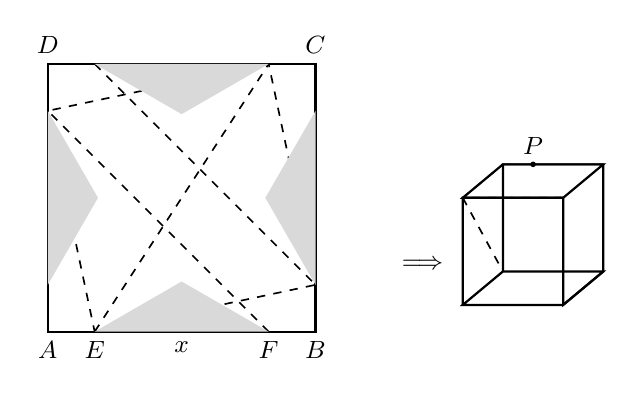
\begin{tikzpicture}[>=stealth, semithick, font=\small, scale=0.85]
  % 左：正方形纸片
  \coordinate (A) at (0,0);
  \coordinate (B) at (4,0);
  \coordinate (C) at (4,4);
  \coordinate (D) at (0,4);
  \coordinate (E) at (0.7,0);
  \coordinate (F) at (3.3,0);
  \coordinate (G) at (4,0.7);
  \coordinate (H) at (3.3,4);
  \coordinate (I) at (0,3.3);
  \coordinate (J) at (0.7,4);
  \draw[thick] (A)--(B)--(C)--(D)--cycle;
  % 折痕
  \draw[dashed] (E)--(G)--(H)--(I)--cycle;
  \draw[dashed] (E)--(H);
  \draw[dashed] (F)--(I);
  \draw[dashed] (J)--(G);
  % 切去的四个等腰直角三角形
  \fill[gray!30] (E)--(F)--(2,0.75)--cycle;
  \fill[gray!30] (J)--(H)--(2,3.25)--cycle;
  \fill[gray!30] (I)--(0.75,2)--(0,0.7)--cycle;
  \fill[gray!30] (G)--(4,3.3)--(3.25,2)--cycle;
  \node[below] at (A) {$A$};
  \node[below] at (B) {$B$};
  \node[above] at (C) {$C$};
  \node[above] at (D) {$D$};
  \node[below] at (E) {$E$};
  \node[below] at (F) {$F$};
  \node[below] at (2,0) {$x$};
  % 右：折成的正四棱柱
  \begin{scope}[xshift=6.2cm, yshift=0.4cm]
    \coordinate (a) at (0,0); \coordinate (b) at (1.5,0);
    \coordinate (c) at (2.1,0.5); \coordinate (d) at (0.6,0.5);
    \coordinate (a1) at (0,1.6); \coordinate (b1) at (1.5,1.6);
    \coordinate (c1) at (2.1,2.1); \coordinate (d1) at (0.6,2.1);
    \draw[thick] (a)--(b)--(c)--(d)--cycle;
    \draw[thick] (a)--(a1)--(b1)--(b)--(c)--(c1)--(d1)--(d);
    \draw[thick] (a1)--(b1)--(c1)--(d1)--cycle;
    \draw[dashed] (d1)--(d);
    \draw[dashed] (a1)--(d);
    \draw[dashed] (b1)--(a1) -- (d1);
    \fill (1.05,2.1) circle (1.2pt) node[above] {$P$};
  \end{scope}
  \node at (5.6,1.0) {$\Longrightarrow$};
\end{tikzpicture}
\end{center}
\nopagebreak[4]
\Needspace{4\baselineskip}
\textbf{解析}
\gksubpart{(1)}
\Needspace{5\baselineskip}
底面边长为 $60-2x$，高为 $x$（$0<x<30$）。侧面积
\nopagebreak[4]
\[S=4x(60-2x)=8x(30-x),\]
当 $x=15$ 时 $S$ 最大（二次函数对称轴 $x=15$）。

\gksubpart{(2)}
\Needspace{5\baselineskip}
容积
\nopagebreak[4]
\[V=x(60-2x)^2=4x(30-x)^2.\]
\Needspace{5\baselineskip}
求导：
\nopagebreak[4]
\[V'=4\left[(30-x)^2-2x(30-x)\right]=4(30-x)(30-3x),\]
故 $0<x<10$ 时 $V'>0$，$10<x<30$ 时 $V'<0$，$x=10$ 时最大。此时底面边长 $60-20=40$，高 $10$，高与底面边长之比为 $\dfrac{10}{40}=\dfrac14$。

\gkanswer{答案（1）：$x=15$。}

\gkanswer{答案（2）：$x=10$，高与底面边长之比为 $\dfrac14$。}

\end{answer}
\begin{answer}
\gksolhead{18}{}

\textbf{题目}：

如图，在平面直角坐标系 $xOy$ 中，$M$，$N$ 分别是椭圆 $\dfrac{x^2}4+\dfrac{y^2}2=1$ 的顶点，过坐标原点的直线交椭圆于 $P$，$A$ 两点，其中点 $P$ 在第一象限，过 $P$ 作 $x$ 轴的垂线，垂足为 $C$，连接 $AC$，并延长交椭圆于点 $B$，设直线 $PA$ 的斜率为 $k$。

（1） 当直线 $PA$ 平分线段 $MN$ 时，求 $k$ 的值；

（2） 当 $k=2$ 时，求点 $P$ 到直线 $AB$ 的距离 $d$；

（3） 对任意 $k>0$，求证：$PA\perp PB$。
\nopagebreak[4]
\begin{center}% 2011 年江苏卷第 18 题：椭圆 x^2/4 + y^2/2 = 1 与点 M,N,P,A,B,C。
% 来源 PDF：普通高考/2011/2011江苏.pdf，SHA-256 71763ef5d0c2b5800c12515e6b3addb77e585b2460fd11c1013fcec6f050ece9。
% 原页：第 1 页第 3 栏下部，书页码 675。按题设取 k=1 示意。
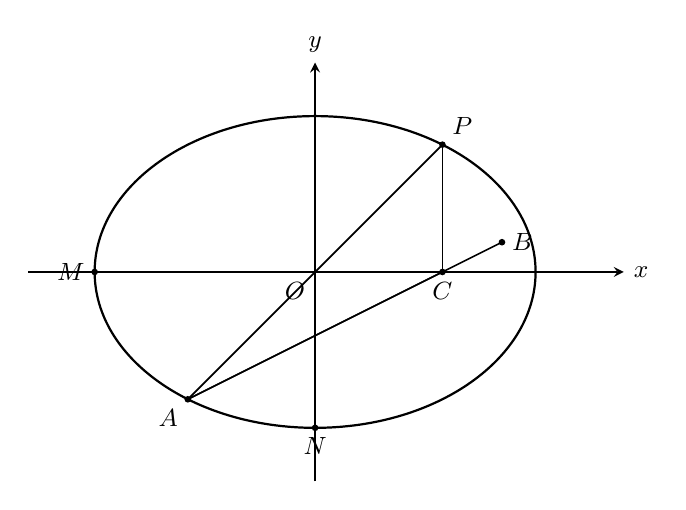
\begin{tikzpicture}[>=stealth, semithick, font=\small, x=1.4cm, y=1.4cm]
  \draw[->] (-2.6,0) -- (2.8,0) node[right] {$x$};
  \draw[->] (0,-1.9) -- (0,1.9) node[above] {$y$};
  \node[below left] at (0,0) {$O$};
  \draw[thick] (0,0) ellipse ({2} and {1.414});
  \coordinate (O) at (0,0);
  \coordinate (M) at (-2,0);
  \coordinate (N) at (0,-1.414);
  \coordinate (P) at (1.155,1.155);
  \coordinate (C) at (1.155,0);
  \coordinate (A) at (-1.155,-1.155);
  \coordinate (B) at (1.695,0.270);
  \draw (P)--(O)--(A);
  \draw (P)--(C);
  \draw (A)--(B);
  \draw (A)--(C);
  \fill (M) circle (1.2pt) node[left] {$M$};
  \fill (N) circle (1.2pt) node[below] {$N$};
  \fill (P) circle (1.2pt) node[above right] {$P$};
  \fill (A) circle (1.2pt) node[below left] {$A$};
  \fill (B) circle (1.2pt) node[right] {$B$};
  \fill (C) circle (1.2pt) node[below] {$C$};
\end{tikzpicture}
\end{center}
\nopagebreak[4]
\Needspace{4\baselineskip}
\textbf{解析}
\gksubpart{(1)}
\Needspace{5\baselineskip}
由椭圆方程，$M(-2,0)$，$N(0,-\sqrt2)$，其中点为 $\left(-1,-\dfrac{\sqrt2}2\right)$。$PA$ 过原点，平分 $MN$ 即 $PA$ 过该中点，故
\nopagebreak[4]
\[k=\frac{-\frac{\sqrt2}2}{-1}=\frac{\sqrt2}2.\]

\gksubpart{(2)}
\Needspace{5\baselineskip}
$k=2$ 时 $P$ 在 $y=2x$ 上，代入椭圆：
\nopagebreak[4]
\[\frac{x^2}4+\frac{4x^2}2=1\Longrightarrow x^2=\frac49,\]
\Needspace{5\baselineskip}
$P\left(\dfrac23,\dfrac43\right)$，$A\left(-\dfrac23,-\dfrac43\right)$，$C\left(\dfrac23,0\right)$。直线 $AC$ 的斜率为 $\dfrac{0-(-4/3)}{2/3-(-2/3)}=1$，即 $AB:y=x-\dfrac23$。点 $P$ 到 $AB$ 的距离
\nopagebreak[4]
\[d=\frac{\left|\frac23-\frac43-\frac23\right|}{\sqrt2}=\frac{4/3}{\sqrt2}=\frac{2\sqrt2}3.\]

\gksubpart{(3)}
\Needspace{5\baselineskip}
设 $P(x_1,y_1)$，$y_1=kx_1$，$x_1^2=\dfrac{4}{1+2k^2}$。直线 $AC$ 过 $A(-x_1,-y_1)$、$C(x_1,0)$，方向向量为 $(2x_1,y_1)$，参数方程
\nopagebreak[4]
\[x=x_1(2t-1),\qquad y=y_1(t-1).\]
\Needspace{5\baselineskip}
代入椭圆：
\nopagebreak[4]
\[\frac{x_1^2(2t-1)^2}4+\frac{y_1^2(t-1)^2}2=1.\]
\Needspace{5\baselineskip}
用 $y_1^2=k^2x_1^2$、$\dfrac1{x_1^2}=\dfrac{1+2k^2}4$，化简得
\nopagebreak[4]
\[t\left[(4+2k^2)t-(4+4k^2)\right]=0,\]
\Needspace{5\baselineskip}
$t=0$ 对应 $A$，故 $B$ 对应 $t=\dfrac{4+4k^2}{4+2k^2}$。于是
\nopagebreak[4]
\[\overrightarrow{PB}=\left(2x_1(t-1),\,y_1(t-2)\right),\qquad \overrightarrow{PA}=(-2x_1,-2y_1).\]
\Needspace{5\baselineskip}
点积
\nopagebreak[4]
\[\overrightarrow{PB}\cdot\overrightarrow{PA}=-4x_1^2(t-1)-2y_1^2(t-2)
=x_1^2\left[(4+4k^2)-t(4+2k^2)\right]=0,\]
故 $PA\perp PB$。

\gkanswer{答案（1）：$k=\dfrac{\sqrt2}2$。}

\gkanswer{答案（2）：$d=\dfrac{2\sqrt2}3$。}

\gkanswer{答案（3）：证明见解析。}

\end{answer}
\begin{answer}
\gksolhead{19}{}

\textbf{题目}：

已知 $a$，$b$ 是实数，函数 $f(x)=x^3+ax$，$g(x)=x^2+bx$，$f'(x)$ 和 $g'(x)$ 分别是 $f(x)$，$g(x)$ 的导函数，若 $f'(x)g'(x)\geqslant0$ 在区间 $I$ 上恒成立，则称 $f(x)$ 和 $g(x)$ 在区间 $I$ 上单调性一致。

（1） 设 $a>0$，若函数 $f(x)$ 和 $g(x)$ 在区间 $[-1,+\infty)$ 上单调性一致，求实数 $b$ 的取值范围；

（2） 设 $a<0$ 且 $a\neq b$，若 $f(x)$ 和 $g(x)$ 在以 $a$，$b$ 为端点的开区间上单调性一致，求 $|a-b|$ 的最大值。

\Needspace{4\baselineskip}
\textbf{解析}
$f'(x)=3x^2+a$，$g'(x)=2x+b$。

\gksubpart{(1)}
$a>0$ 时 $f'(x)>0$ 恒成立，故只需 $g'(x)\geqslant0$ 在 $[-1,+\infty)$ 上恒成立。$g'$ 递增，最小值在 $x=-1$：$g'(-1)=-2+b\geqslant0$，即 $b\geqslant2$。

\gksubpart{(2)}
$a<0$ 时 $f'$ 在 $\left(-\sqrt{-\frac a3},\sqrt{-\frac a3}\right)$ 上为负、在其外为正；$g'$ 在 $\left(-\infty,-\dfrac b2\right)$ 为负、在 $\left(-\dfrac b2,+\infty\right)$ 为正。
设区间端点为 $a<b$（另一情形同理）。若 $b\geqslant0$，区间含 $0$，在 $0$ 附近 $f'<0$、$g'>0$，乘积为负，不成立，故 $b<0$。此时 $-\dfrac b2>0$，在 $(a,b)$ 上 $g'<0$，需 $f'<0$，即 $(a,b)\subset\left(-\sqrt{-\frac a3},\sqrt{-\frac a3}\right)$。因 $b<0$，只需 $a\geqslant-\sqrt{-\frac a3}$。令 $u=-a>0$，则 $u\leqslant\sqrt{u/3}$，即 $u\leqslant\dfrac13$。
于是 $|a-b|=b-a<0+u\leqslant\dfrac13$（$b<0$）。当 $a=-\dfrac13$、$b\to0^-$ 时趋近 $\dfrac13$，故最大值为 $\dfrac13$。

\gkanswer{答案（1）：$b\geqslant2$。}

\gkanswer{答案（2）：$\dfrac13$。}

\end{answer}
\begin{answer}
\gksolhead{20}{}

\textbf{题目}：

设 $M$ 为部分正整数组成的集合，数列 $\{a_n\}$ 的首项 $a_1=1$，前 $n$ 项和为 $S_n$，已知对任意整数 $k\in M$，当整数 $n>k$ 时，$S_{n+k}+S_{n-k}=2(S_n+S_k)$ 都成立。

（1） 设 $M=\{1\}$，$a_2=2$，求 $a_5$ 的值；

（2） 设 $M=\{3,4\}$，求数列 $\{a_n\}$ 的通项公式。

\Needspace{4\baselineskip}
\textbf{解析}
\gksubpart{(1)}
\Needspace{5\baselineskip}
$k=1$ 时，对 $n>1$，
\nopagebreak[4]
\[S_{n+1}+S_{n-1}=2S_n+2S_1\Longrightarrow a_{n+1}-a_n=2S_1=2.\]
故从 $a_2=2$ 起公差为 $2$：$a_3=4$，$a_4=6$，$a_5=8$。

\gksubpart{(2)}
\Needspace{5\baselineskip}
分别取 $k=3$、$k=4$，对 $n>4$ 有
\nopagebreak[4]
\[a_{n+1}+a_{n+2}+a_{n+3}=a_{n-2}+a_{n-1}+a_n+2S_3,\tag{1}\]
\nopagebreak[4]
\[a_{n+1}+a_{n+2}+a_{n+3}+a_{n+4}=a_{n-3}+a_{n-2}+a_{n-1}+a_n+2S_4.\tag{2}\]
\gksubpart{(2)}
\Needspace{5\baselineskip}
减（1）得
\nopagebreak[4]
\[a_{n+4}-a_{n-3}=2(S_4-S_3)=2a_4.\]
\Needspace{5\baselineskip}
又对（1）取 $n$ 与 $n+1$ 相减，得
\nopagebreak[4]
\[a_{n+4}+a_{n-2}=2a_{n+1}.\]
\Needspace{5\baselineskip}
由这两式可消去 $a_{n+4}$，整理得 $a_{n+2}-a_{n+1}=a_{n+1}-a_n$，故 $\{a_n\}$ 为等差数列。设公差为 $d$，由 $k=3,n=4$：
\nopagebreak[4]
\[S_7+S_1=2S_4+2S_3.\]
代入 $S_n=n+\dfrac{n(n-1)}2d$：左边 $7+21d+1$，右边 $2(4+6d)+2(3+3d)=14+18d$，得 $8+21d=14+18d$，$d=2$。故 $a_n=1+2(n-1)=2n-1$。
验证：$a_n=2n-1$ 时 $S_n=n^2$，对 $k=3,4$ 均有 $(n+k)^2+(n-k)^2=2(n^2+k^2)$，满足条件。

\gkanswer{答案（1）：$a_5=8$。}

\gkanswer{答案（2）：$a_n=2n-1$。}

\end{answer}
\begin{answer}
\gksolhead{21}{}

\textbf{题目}：

四选二。

【A】如图，圆 $O_1$ 与圆 $O_2$ 内切于点 $A$，其半径分别为 $r_1$ 与 $r_2$（$r_1>r_2$），圆 $O_1$ 的弦 $AB$ 交圆 $O_2$ 于点 $C$（$O_1$ 不在 $AB$ 上），求证：$AB:AC$ 为定值。
\nopagebreak[4]
\begin{center}% 2011 年江苏卷附加题 21A：两圆内切于点 A，圆 O1 的弦 AB 交圆 O2 于 C。
% 来源 PDF：普通高考/2011/2011江苏.pdf，SHA-256 71763ef5d0c2b5800c12515e6b3addb77e585b2460fd11c1013fcec6f050ece9。
% 原页：第 2 页第 2 栏，书页码 676。r1:r2 示意取 2.2:1.3。
\begin{tikzpicture}[>=stealth, semithick, font=\small, scale=0.9]
  \coordinate (O1) at (0,0);
  \coordinate (O2) at (0.9,0);
  \coordinate (A) at (2.2,0);
  \coordinate (B) at (-1.1,1.905);
  \draw[thick] (O1) circle (2.2);
  \draw[thick] (O2) circle (1.3);
  \draw (A)--(B);
  \fill (O1) circle (1.2pt) node[below] {$O_1$};
  \fill (O2) circle (1.2pt) node[below] {$O_2$};
  \fill (A) circle (1.2pt) node[right] {$A$};
  \fill (B) circle (1.2pt) node[above left] {$B$};
  \coordinate (C) at ($(A)!0.56!(B)$);
  \fill (C) circle (1.2pt) node[below right] {$C$};
\end{tikzpicture}
\end{center}
\nopagebreak[4]
【B】已知矩阵 $A=\begin{bmatrix}1&1\\2&1\end{bmatrix}$，向量 $\boldsymbol\beta=\begin{bmatrix}1\\2\end{bmatrix}$，求向量 $\boldsymbol\alpha$，使得 $A^2\boldsymbol\alpha=\boldsymbol\beta$。

【C】在平面直角坐标系 $xOy$ 中，求过椭圆 $\begin{cases}x=5\cos\varphi,\\y=3\sin\varphi\end{cases}$（$\varphi$ 为参数）的右焦点，且与直线 $\begin{cases}x=4-2t,\\y=3-t\end{cases}$（$t$ 为参数）平行的直线的普通方程。

【D】解不等式：$x+|2x-1|<3$。

\Needspace{4\baselineskip}
\textbf{解析}
\Needspace{5\baselineskip}
【A】以 $A$ 为位似中心、比 $k=\dfrac{r_2}{r_1}$ 作位似变换，圆 $O_1$ 变为圆 $O_2$。点 $B$ 在圆 $O_1$ 上，其像 $B'$ 在射线 $AB$ 上且 $AB'=k\cdot AB$，同时在圆 $O_2$ 上。射线 $AB$ 与圆 $O_2$ 的另一交点正是 $C$，故 $B'=C$，$AC=k\cdot AB$。于是
\nopagebreak[4]
\[\frac{AB}{AC}=\frac{r_1}{r_2},\]
为定值。

\Needspace{5\baselineskip}
【B】$A^2=\begin{bmatrix}1&1\\2&1\end{bmatrix}^2=\begin{bmatrix}3&2\\4&3\end{bmatrix}$。设 $\boldsymbol\alpha=\begin{bmatrix}x\\y\end{bmatrix}$，则
\nopagebreak[4]
\[\begin{cases}3x+2y=1,\\4x+3y=2.\end{cases}\]
两式相减得 $x+y=1$，代回第一式得 $x=-1$，$y=2$。故 $\boldsymbol\alpha=\begin{bmatrix}-1\\2\end{bmatrix}$。

\Needspace{5\baselineskip}
【C】椭圆 $\dfrac{x^2}{25}+\dfrac{y^2}9=1$ 的右焦点为 $(4,0)$。参数直线消去 $t$：由 $x=4-2t$、$y=3-t$ 得 $x-2y+2=0$，斜率为 $\dfrac12$。所求直线过 $(4,0)$ 且斜率 $\dfrac12$：
\nopagebreak[4]
\[y=\frac12(x-4)\Longrightarrow x-2y-4=0.\]

【D】当 $x\geqslant\dfrac12$ 时，$x+2x-1<3$，即 $x<\dfrac43$，得 $\dfrac12\leqslant x<\dfrac43$；当 $x<\dfrac12$ 时，$x+1-2x<3$，即 $x>-2$，得 $-2<x<\dfrac12$。合并得解集 $\left(-2,\dfrac43\right)$。

\gkanswer{答案：A 证明见解析（$AB:AC=r_1:r_2$）；B $\boldsymbol\alpha=\begin{bmatrix}-1\\2\end{bmatrix}$；C $x-2y-4=0$；D $\left(-2,\dfrac43\right)$。}

\end{answer}
\begin{answer}
\gksolhead{22}{}

\textbf{题目}：

如图，在正四棱柱 $ABCD-A_1B_1C_1D_1$ 中，$AA_1=2$，$AB=1$，点 $N$ 是 $BC$ 的中点，点 $M$ 在 $CC_1$ 上。设二面角 $A_1-DN-M$ 的大小为 $\theta$。

（1） 当 $\theta=90^\circ$ 时，求 $AM$ 的长；

（2） 当 $\cos\theta=\dfrac{\sqrt6}6$ 时，求 $CM$ 的长。
\nopagebreak[4]
\begin{center}% 2011 年江苏卷附加题 22：正四棱柱 ABCD-A1B1C1D1，N 为 BC 中点，M 在 CC1 上。
% 来源 PDF：普通高考/2011/2011江苏.pdf，SHA-256 71763ef5d0c2b5800c12515e6b3addb77e585b2460fd11c1013fcec6f050ece9。
% 原页：第 2 页第 3 栏，书页码 676。AA1=2，AB=1，示意不按比例。
\begin{tikzpicture}[>=stealth, semithick, font=\small, scale=0.95]
  \coordinate (A) at (0,0);
  \coordinate (B) at (2.0,0.15);
  \coordinate (C) at (2.8,1.05);
  \coordinate (D) at (0.8,0.9);
  \coordinate (A1) at (0.35,2.5);
  \coordinate (B1) at (2.35,2.65);
  \coordinate (C1) at (3.15,3.55);
  \coordinate (D1) at (1.15,3.4);
  \coordinate (N) at ($(B)!0.5!(C)$);
  \coordinate (M) at ($(C)!0.45!(C1)$);
  \draw[thick] (A)--(B)--(C)--(D)--cycle;
  \draw[thick] (A)--(A1) (B)--(B1) (C)--(C1) (D)--(D1);
  \draw[thick] (A1)--(B1)--(C1)--(D1)--cycle;
  \draw[dashed] (A1)--(D);
  \draw[dashed] (D)--(D1);
  \draw[dashed] (A1)--(D1);
  \draw (A1)--(N);
  \draw (D)--(N);
  \draw (D)--(M);
  \draw (N)--(M);
  \fill (N) circle (1.2pt) node[below right] {$N$};
  \fill (M) circle (1.2pt) node[right] {$M$};
  \node[below left] at (A) {$A$};
  \node[below] at (B) {$B$};
  \node[right] at (C) {$C$};
  \node[left] at (D) {$D$};
  \node[left] at (A1) {$A_1$};
  \node[above] at (B1) {$B_1$};
  \node[right] at (C1) {$C_1$};
  \node[above] at (D1) {$D_1$};
\end{tikzpicture}
\end{center}
\nopagebreak[4]
\Needspace{4\baselineskip}
\textbf{解析}
\Needspace{5\baselineskip}
以 $A$ 为原点，$AB$、$AD$、$AA_1$ 为坐标轴建立空间直角坐标系，则
\nopagebreak[4]
\[A(0,0,0),\ B(1,0,0),\ D(0,1,0),\ C(1,1,0),\ A_1(0,0,2),\]
$N$ 为 $BC$ 中点，$N\left(1,\dfrac12,0\right)$；设 $M(1,1,m)$（$0\leqslant m\leqslant2$）。
\Needspace{5\baselineskip}
平面 $A_1DN$ 的法向量：$\overrightarrow{DN}=\left(1,-\dfrac12,0\right)$，$\overrightarrow{DA_1}=(0,-1,2)$，
\nopagebreak[4]
\[\boldsymbol n_1=\overrightarrow{DN}\times\overrightarrow{DA_1}=(-1,-2,-1),\]
取 $\boldsymbol n_1=(1,2,1)$。
\Needspace{5\baselineskip}
平面 $DNM$ 的法向量：$\overrightarrow{DN}=\left(1,-\dfrac12,0\right)$，$\overrightarrow{DM}=(1,0,m)$，
\nopagebreak[4]
\[\boldsymbol n_2=\overrightarrow{DN}\times\overrightarrow{DM}=\left(-\frac m2,-m,\frac12\right),\]
取 $\boldsymbol n_2=(-m,-2m,1)$。
\gksubpart{(1)}
\Needspace{5\baselineskip}
$\theta=90^\circ$ 时 $\boldsymbol n_1\cdot\boldsymbol n_2=0$：
\nopagebreak[4]
\[-m-4m+1=0\Longrightarrow m=\frac15.\]
\Needspace{5\baselineskip}
此时 $M\left(1,1,\dfrac15\right)$，
\nopagebreak[4]
\[AM=\sqrt{1^2+1^2+\left(\frac15\right)^2}=\frac{\sqrt{51}}5.\]

\gksubpart{(2)}
\Needspace{5\baselineskip}
$\cos\theta=\dfrac{|\boldsymbol n_1\cdot\boldsymbol n_2|}{|\boldsymbol n_1||\boldsymbol n_2|}=\dfrac{|1-5m|}{\sqrt6\sqrt{5m^2+1}}=\dfrac{\sqrt6}6$。平方得
\nopagebreak[4]
\[\frac{(1-5m)^2}{6(5m^2+1)}=\frac16\Longrightarrow(1-5m)^2=5m^2+1,\]
即 $20m^2-10m=0$，$m=\dfrac12$（$m=0$ 时二面角为 $0$，舍去）。故 $CM=\dfrac12$。

\gkanswer{答案（1）：$AM=\dfrac{\sqrt{51}}5$。}

\gkanswer{答案（2）：$CM=\dfrac12$。}

\end{answer}
\begin{answer}
\gksolhead{23}{}

\textbf{题目}：

设整数 $n\geqslant4$，$P(a,b)$ 是平面直角坐标系 $xOy$ 中的点，其中 $a$，$b\in\{1,2,3,\cdots,n\}$，$a>b$。

（1） 记 $A_n$ 为满足 $a-b=3$ 的点 $P$ 的个数，求 $A_n$；

（2） 记 $B_n$ 为满足 $\dfrac13(a-b)$ 是整数的点 $P$ 的个数，求 $B_n$。

\Needspace{4\baselineskip}
\textbf{解析}
\gksubpart{(1)}
$a=b+3$，$b=1,2,\cdots,n-3$，故 $A_n=n-3$。

\gksubpart{(2)}
\Needspace{5\baselineskip}
对每个 $d=a-b\in\{1,2,\cdots,n-1\}$，满足 $a-b=d$ 的点有 $n-d$ 个。$B_n$ 只计 $3\mid d$ 的情形：
\nopagebreak[4]
\[B_n=\sum_{\substack{1\leqslant d\leqslant n-1\\3\mid d}}(n-d).\]
写 $n=3q+r$（$r=0,1,2$）。
\Needspace{5\baselineskip}
$r=0$ 时，$d=3,6,\cdots,3(q-1)$，共 $q-1$ 项，
\nopagebreak[4]
\[B_n=(q-1)n-3\cdot\frac{(q-1)q}2=\frac{3q(q-1)}2=\frac{n(n-3)}6.\]
\Needspace{5\baselineskip}
$r=1$ 或 $2$ 时，$d=3,6,\cdots,3q$，共 $q$ 项，
\nopagebreak[4]
\[B_n=qn-3\cdot\frac{q(q+1)}2=\frac{q(3q-1)}2=\frac{(n-1)(n-2)}6.\]
\Needspace{5\baselineskip}
故
\nopagebreak[4]
\[B_n=\begin{cases}\dfrac{n(n-3)}6,&3\mid n,\\[4pt]\dfrac{(n-1)(n-2)}6,&3\nmid n.\end{cases}\]

\gkanswer{答案（1）：$A_n=n-3$。}

\gkanswer{答案（2）：$B_n=\begin{cases}\dfrac{n(n-3)}6,&3\mid n,\\[4pt]\dfrac{(n-1)(n-2)}6,&3\nmid n.\end{cases}$}

\end{answer}